\documentclass[a4paper,10pt,french]{article}
\linespread{1}

\title{Chapitre 3 : G\'eom\'etrie dans l'espace }
\author{D. Zancanaro \and C. Aup\'erin}
\date{2009-2010}
\usepackage{pifont}

%%%%%%%%%%%%%%%%%%%%%%%%%%%%%%%%%%%%%%%%%%%%%%%%%%%%%%%%%%%%%%%%%%%%%%%		Packages

\newcommand{\ch}{Chapitre 3}
\newcommand{\Ch}{G\'eom\'etrie \linebreak[2] dans l'espace}	
\newcommand{\Cl}{2$^{\text{nde}}$}	
\newcommand{\Annee}{2010-2011}	
%%%%%%%%%%%%%%%%%%%%%%%%%%%%%%%%%%%%%%%%%%%%%%%%%%%%%%%%%%%%%%%%%%%%%%%		Package
%\usepackage[french,lined,boxed,commentsnumbered]{algorithm2e}

\input macro_dwicky_final.tex

\geometry{hmargin=2cm,vmargin=2.5cm}

\setcounter{NumLecon}{3}
%%%%%%%%%%%%%%%%%%%%%%%%%%%%%%%%%%%%%%%%%%%%%%%%%%%%%%%%%%%%%%%%%%%	Premiere page
\begin{document}
%%%%%%%%%%%%%%%%%%%%%%%%%%%%%%%%%%%%%%%%%%%%%%%%%%%%%%%%%%%%%%%%%%%%%%%%	Cadre jaune
\begin{center}
\includegraphics[scale=1]{pyramide.eps}		
\end{center}

\begin{center}
\psset{xunit=1.0cm,yunit=1.0cm,algebraic=true,dotstyle=o,dotsize=3pt 0,linewidth=0.8pt,arrowsize=3pt 2,arrowinset=0.25}
\begin{pspicture*}(-3.71,-0.25)(6.98,7.16)
\psline(-0.2,0.95)(4.42,3.29)
\psline(0.08,6.12)(-0.2,0.95)
\psline(0.08,6.12)(4.42,3.29)
\psline(0.08,6.12)(1.43,3.45)
\psline(1.43,3.45)(-0.2,0.95)
\psline(1.43,3.45)(4.42,3.29)
\pscircle[linestyle=dotted](0.08,6.12){2.59}
\pscircle[linestyle=dotted](4.42,3.29){2.59}
\pscircle[linestyle=dotted](-0.2,0.95){2.59}
\psline(-0.2,0.95)(-0.06,3.54)
\pscircle[linestyle=dotted](1.43,3.45){2.59}
\psdots[dotsize=1pt 0,dotstyle=*](-0.2,0.95)
\rput[bl](-0.45,0.66){$A$}
\psdots[dotsize=1pt 0,dotstyle=*](4.42,3.29)
\rput[bl](4.61,3.16){$B$}
\psdots[dotsize=1pt 0,dotstyle=*](2.11,2.12)
\rput[bl](2.26,1.86){$C'$}
\psdots[dotsize=1pt 0,dotstyle=*](0.08,6.12)
\rput[bl](0.07,6.21){$C$}
\psdots[dotsize=1pt 0,dotstyle=*](2.25,4.71)
\rput[bl](2.31,4.74){$A'$}
\psdots[dotsize=1pt 0,dotstyle=*](-0.06,3.54)
\rput[bl](-0.42,3.29){$B'$}
\psdots[dotsize=1pt 0,dotstyle=*](1.43,3.45)
\rput[bl](1.39,3.6){$D$}
\end{pspicture*}
\end{center}

\begin{center}
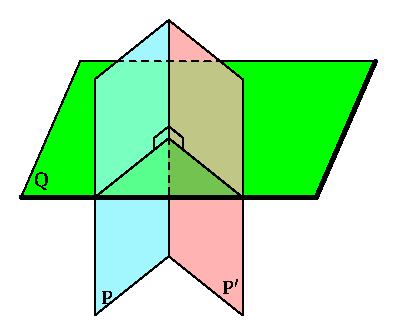
\includegraphics[scale=1]{fig2c_espace.1}		
\end{center}

\begin{center}
\includegraphics[scale=0.6]{cavalier.eps}		
\end{center}

\begin{center}
\includegraphics[scale=0.6]{cavalier2.eps}		
\end{center}

\begin{tabular}{ccc}
	 trois points non alignés & deux droites sécantes & une droite et un 
	 point extérieur à celle-ci \\
	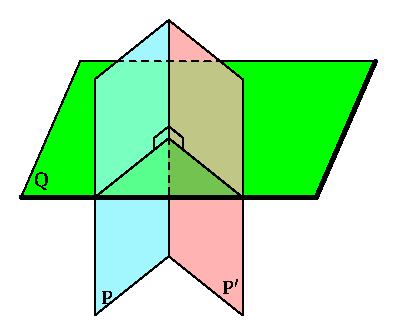
\includegraphics[scale=1]{fig2c_espace.3}	 	
		  & 
	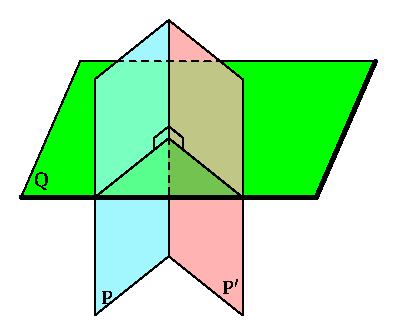
\includegraphics[scale=1]{fig2c_espace.4}	 	
	      &
	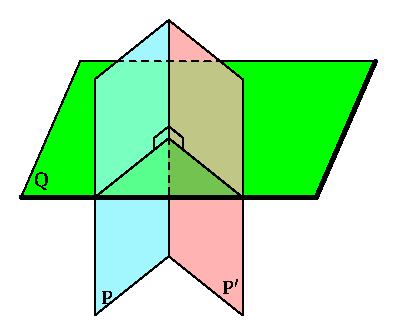
\includegraphics[scale=1]{fig2c_espace.5}	 	 	
	       \\
\end{tabular}

\begin{center}
\psset{xunit=1.0cm,yunit=1.0cm,algebraic=true,dotstyle=o,dotsize=3pt 0,linewidth=0.8pt,arrowsize=3pt 2,arrowinset=0.25}
\begin{pspicture*}(-1,-1)(8.5,7)
\psline(0,4.5)(2,5.5)
\psline(4,0)(6,1)
\psline[linestyle=dotted](0,0.5)(2,1.5)
\psplot{-1}{8}{(--2-0.5*x)/4}
\psline(4,4)(6,5)
\psline(0,4.5)(4,4)
\psline(4,4)(4,0)
\psline(0,0.5)(4,0)
\psline(0,0.5)(0,4.5)
\psline(6,5)(2,5.5)
\psline(6,5)(6,1)
\psline[linestyle=dotted](2,1.5)(2,5.5)
\psline[linestyle=dotted](2,1.5)(6,1)
\psplot{-1}{8}{(--18-2.5*x)/4}
\rput[bl](3.74,4.14){$B$}
\rput[bl](3.96,-0.34){$C$}
\rput[bl](1.66,5.66){$E$}
\rput[bl](5.82,5.14){$F$}
\rput[bl](6.24,0.9){$G$}
\rput[bl](1.56,1.42){$H$}
\rput[bl](-0.24,4.68){$A$}
\rput[bl](-0.34,0.2){$D$}
\rput[bl](4.08,2.12){$I$}
\rput[bl](8.08,-0.38){$J$}
\end{pspicture*}
\end{center}


\pagebreak

\begin{minipage}{9cm}
\psset{unit=0.8}
   \begin{center}
      Parallélpipède rectangle : $V =L\times$l$\times$ h. \\
      \begin{pspicture}(0,-1.2)(5,3.5)
         \pspolygon(0,0)(4,0)(5,1)(5,3)(1,3)(0,2)
         \psline(0,2)(4,2)(4,0)
         \psline(4,2)(5,3)
         \psline[linestyle=dashed](0,0)(1,1)(5,1)
         \psline[linestyle=dashed](1,1)(1,3)
      \end{pspicture} \\
      Sphère : V= $\dfrac{4}{3}\times\pi\times r^3$ \\
      \begin{pspicture}(-1,-1)(5,5.2)
         \pscircle(2.5,2.5){2.5}
         \psellipticarc[linestyle=dashed](2.5,2.5)(2.5,1){0}{180}
         \psellipticarc(2.5,2.5)(2.5,1){180}{0}
         \rput(2.5,2.1){$O$}
         \psline[linestyle=dashed,linecolor=blue]{<->}(2.5,2.5)(5,2.5)
         \psdot(2.5,2.5)
         \rput(3.75,2.2){\textcolor{blue}{$r$}}
      \end{pspicture} \\
      Cylindre de révolution : $V =\pi\times r^2\times h$. \\
      \begin{pspicture}(-2,0)(5,6.5)
         \psline(4,1)(4,5)
         \psline(0,1)(0,5)
         \psellipse(2,5)(2,1)
         \psellipticarc(2,1)(2,1){180}{0}
         \psellipticarc[linestyle=dashed](2,1)(2,1){0}{180} 
         \psline[linewidth=0.05,linecolor=blue]{<->}(2,1)(4,1)
         \rput(3,1.2){\textcolor{blue}{$r$}}
         \psline[linewidth=0.05,linecolor=blue]{|-|}(5,1)(5,5)  
         \rput(5.3,3){\textcolor{blue}{$h$} }
      \end{pspicture}
   \end{center}
\end{minipage}
\begin{minipage}{9cm}
\psset{unit=0.8}
   \begin{center}
   pyramide : $V =\dfrac{\text{aire de la base}\times\text{h}}{3}$. \\
      \begin{pspicture}(-0.5,-1.5)(5,6.5)
         \pspolygon(1,0)(4,0)(5,1)(2.5,6)(0,1)
         \psline(1,0)(2.5,6)(4,0)
         \psline[linestyle=dashed](0,1)(1.3,2)(3.7,2)(5,1)
         \psline[linestyle=dashed](1.3,2)(2.5,6)
         \psline[linestyle=dashed](3.7,2)(2.5,6)
         \psline[linewidth=0.05,linecolor=blue](2.5,6)(2.5,1)
         \psline[linewidth=0.05,linecolor=blue](2.8,1)(2.8,1.3)(2.5,1.3)
         \rput(2.7,2.8){\textcolor{blue}{$h$}}
      \end{pspicture} \\
      Cône de révolution : $V =\dfrac{\pi\times r^2\times h}{3}$. \\
      \begin{pspicture}(-1.8,0)(5,6.5)
         \psline(4,1)(2,6)(0,1)
         \psellipticarc(2,1)(2,1){180}{0}
         \psellipticarc[linestyle=dashed](2,1)(2,1){0}{180} 
         \psline[linewidth=0.05,linecolor=blue](2,1)(2,6)
         \rput(2.5,3.5){\textcolor{blue}{$h$}}
         \psline[linewidth=0.05,linecolor=blue]{<->}(2,1)(4,1)
         \rput(3,1.2){\textcolor{blue}{$r$}}
      \end{pspicture}
   \end{center}
\end{minipage}

\begin{multicols}{2}
\Exop{Soit $ABCDEFGH$ un cube d'arête $4$ cm. Soit $I$, $J$ et $M$ les milieux respectifs de $[BC]$, $[AB]$ et $[BF]$.
\begin{enumerate}
\item Quelle est la nature du triangle $IJM$ ? Le représenter en vraie grandeur.
\item Calculer le volume du tétraèdre $BIJM$.
\item On enlève les huit \og coins \fg du cube pour obtenir le solide représenté ci-contre, appelé \og cuboctaèdre \fg.
\begin{enumerate}
\item Combien de faces ce solide comporte-t-il ? Quelle est la nature de ces faces ?
\item Calculer le volume exact de ce cuboctaèdre, puis en donner une valeur approchée au centimètre cube près.
\end{enumerate}
\end{enumerate}}
\begin{center}
\newrgbcolor{zzttqq}{0.6 0.2 0}
\newrgbcolor{ffzzzz}{1 0.6 0.6}
\psset{xunit=1.0cm,yunit=1.0cm,algebraic=true,dotstyle=o,dotsize=3pt 0,linewidth=0.8pt,arrowsize=3pt 2,arrowinset=0.25}
\begin{pspicture*}(-0.34,-0.36)(7.54,7.54)
\pspolygon[linestyle=none,fillstyle=solid,fillcolor=ffzzzz,opacity=0.1](4,2)(2,0.25)(5,0.5)
\pspolygon[linestyle=none,fillstyle=solid,fillcolor=ffzzzz,opacity=0.1](2,4.25)(4,2)(5,4.5)
\pspolygon[linestyle=none,fillstyle=solid,fillcolor=ffzzzz,opacity=0.1](2,4.25)(0,2.5)(1,5)
\pspolygon[linestyle=none,fillstyle=solid,fillcolor=ffzzzz,opacity=0.1](0,2.5)(2,0.25)(1,1)
\pspolygon[linestyle=none,fillstyle=solid,fillcolor=ffzzzz,opacity=0.1](1,5)(2,3.5)(4,5.25)
\pspolygon[linestyle=none,fillstyle=solid,fillcolor=zzttqq,opacity=0.9](0,2.5)(2,4.25)(4,2)(2,0.25)
\pspolygon[linestyle=none,fillstyle=solid,fillcolor=zzttqq,opacity=0.9](2,4.25)(1,5)(4,5.25)(5,4.5)
\pspolygon[linestyle=none,fillstyle=solid,fillcolor=zzttqq,opacity=0.9](5,4.5)(4,2)(5,0.5)(6,3)
%\pspolygon[linestyle=none,fillstyle=solid,fillcolor=zzttqq,opacity=0.1](0,2.5)(1,5)(2,3.5)(1,1)
%\pspolygon[linestyle=none,fillstyle=solid,fillcolor=zzttqq,opacity=0.1](1,1)(2,0.25)(5,0.5)(4,1.25)
%\pspolygon[linestyle=none,fillstyle=solid,fillcolor=zzttqq,opacity=0.1](2,3.5)(4,5.25)(6,3)(4,1.25)
\psline(0,4.5)(2,5.5)
\psline(4,0)(6,1)
\psline[linestyle=dotted](0,0.5)(2,1.5)
\psline(4,4)(6,5)
\psline(0,4.5)(4,4)
\psline(4,4)(4,0)
\psline(0,0.5)(4,0)
\psline(0,0.5)(0,4.5)
\psline(6,5)(2,5.5)
\psline(6,5)(6,1)
\psline[linestyle=dotted](2,1.5)(2,5.5)
\psline[linestyle=dotted](2,1.5)(6,1)
\psline[linecolor=ffzzzz](4,2)(2,0.25)
\psline[linecolor=ffzzzz](2,0.25)(5,0.5)
\psline[linecolor=ffzzzz](5,0.5)(4,2)
\psline[linecolor=ffzzzz](2,4.25)(4,2)
\psline[linecolor=ffzzzz](4,2)(5,4.5)
\psline[linecolor=ffzzzz](5,4.5)(2,4.25)
\psline[linecolor=ffzzzz](2,4.25)(0,2.5)
\psline[linecolor=ffzzzz](0,2.5)(1,5)
\psline[linecolor=ffzzzz](1,5)(2,4.25)
\psline[linecolor=ffzzzz](0,2.5)(2,0.25)
\psline[linecolor=ffzzzz](2,0.25)(1,1)
\psline[linecolor=ffzzzz](1,1)(0,2.5)
\psline[linecolor=ffzzzz](1,5)(2,3.5)
\psline[linecolor=ffzzzz](2,3.5)(4,5.25)
\psline[linecolor=ffzzzz](4,5.25)(1,5)
\psline[linecolor=zzttqq](0,2.5)(2,4.25)
\psline[linecolor=zzttqq](2,4.25)(4,2)
\psline[linecolor=zzttqq](4,2)(2,0.25)
\psline[linecolor=zzttqq](2,0.25)(0,2.5)
\psline[linecolor=zzttqq](2,4.25)(1,5)
\psline[linecolor=zzttqq](1,5)(4,5.25)
\psline[linecolor=zzttqq](4,5.25)(5,4.5)
\psline[linecolor=zzttqq](5,4.5)(2,4.25)
\psline[linecolor=zzttqq](5,4.5)(4,2)
\psline[linecolor=zzttqq](4,2)(5,0.5)
\psline[linecolor=zzttqq](5,0.5)(6,3)
\psline[linecolor=zzttqq](6,3)(5,4.5)
\psline[linecolor=zzttqq](0,2.5)(1,5)
\psline[linecolor=zzttqq](1,5)(2,3.5)
\psline[linecolor=zzttqq](2,3.5)(1,1)
\psline[linecolor=zzttqq](1,1)(0,2.5)
\psline[linecolor=zzttqq](1,1)(2,0.25)
\psline[linecolor=zzttqq](2,0.25)(5,0.5)
\psline[linecolor=zzttqq](5,0.5)(4,1.25)
\psline[linecolor=zzttqq](4,1.25)(1,1)
\psline[linecolor=zzttqq](2,3.5)(4,5.25)
\psline[linecolor=zzttqq](4,5.25)(6,3)
\psline[linecolor=zzttqq](6,3)(4,1.25)
\psline[linecolor=zzttqq](4,1.25)(2,3.5)
\rput[bl](3.74,4.14){$B$}
\rput[bl](3.96,-0.34){$C$}
\rput[bl](1.66,5.66){$E$}
\rput[bl](5.82,5.14){$F$}
\rput[bl](6.24,0.9){$G$}
\rput[bl](1.56,1.42){$H$}
\rput[bl](-0.24,4.68){$A$}
\rput[bl](-0.34,0.2){$D$}
\rput[bl](4.08,2.12){$I$}
\rput[bl](2.08,4.36){$J$}
%\rput[bl](4.08,5.36){\darkgray{$K$}}
%\rput[bl](1.08,5.12){\darkgray{$L$}}
\rput[bl](5.08,4.62){$M$}
%\rput[bl](6.08,3.12){\darkgray{$N$}}
%\rput[bl](5.08,0.62){\darkgray{$O$}}
%\rput[bl](2.08,0.36){\darkgray{$P$}}
%\rput[bl](1.08,1.12){\darkgray{$Q$}}
%\rput[bl](4.08,1.36){\darkgray{$R$}}
%\rput[bl](2.08,3.62){\darkgray{$S$}}
%\rput[bl](0.08,2.62){\darkgray{$T$}}
\end{pspicture*}
\end{center}
\end{multicols}

\pagebreak

	   \begin{center}
	    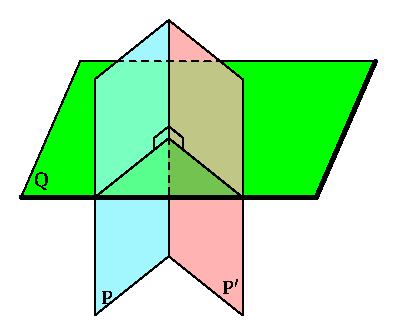
\includegraphics[scale=1]{fig2c_espace.7}		
	   \end{center}
	   
	   	   \begin{center}
	 \begin{tabular}{cc}
	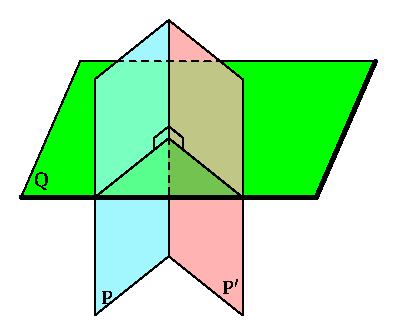
\includegraphics[scale=1]{fig2c_espace.4}	 	
	      &
	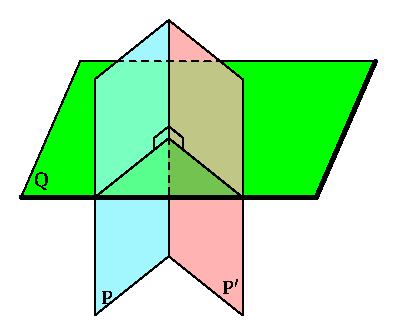
\includegraphics[scale=1]{fig2c_espace.6}	 	 	
	       \\
	        deux droites sécantes & deux droites parallèles\\
\end{tabular}
\end{center}

	\begin{center}
			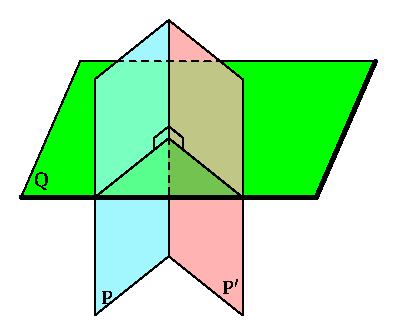
\includegraphics[scale=1]{fig2c_espace.20}	 
			\end{center}
			
				\begin{center}
	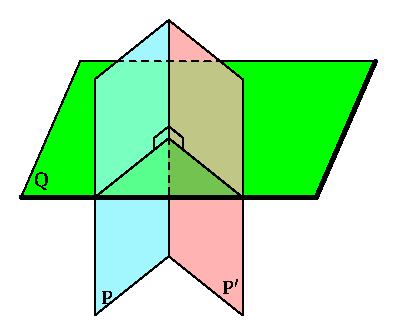
\includegraphics[scale=1]{fig2c_espace.2}		
	\end{center}
	
		\begin{center}
	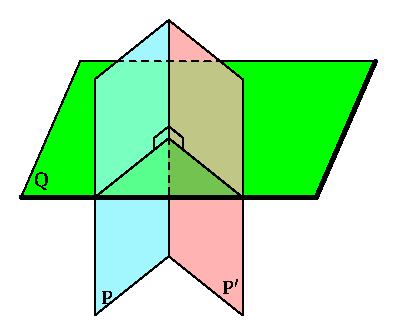
\includegraphics[scale=1]{fig2c_espace.19}		
	\end{center}
	
			\begin{center}
			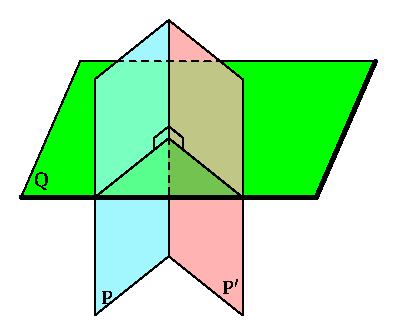
\includegraphics[scale=1]{fig2c_espace.21}	 
			\end{center}
			
			\begin{center}
\psset{xunit=0.8cm,yunit=0.8cm,algebraic=true,dotstyle=o,dotsize=3pt 0,linewidth=0.8pt,arrowsize=3pt 2,arrowinset=0.25}
\begin{pspicture*}(2,-2)(8.6,4.4)
\psline[linewidth=1.2pt](2.5,-1.4)(6.7,-1.7)
\psline[linewidth=1.2pt](6.7,-1.7)(7.9,0.5)
\psline[linewidth=1.2pt,linestyle=dotted](2.5,-1.4)(7.9,0.5)
\psline[linewidth=1.2pt](6.7,-1.7)(4.2,3.8)
\psline[linewidth=1.2pt](4.2,3.8)(2.5,-1.4)
\psline[linewidth=1.2pt](4.2,3.8)(7.9,0.5)
\rput[bl](2.1,-1.6){$A$}
\rput[bl](6.9,-2){$B$}
\rput[bl](7.9,0.6){$C$}
\rput[bl](4.3,4){$D$}
\rput[bl](4.7,-1.4){$I$}
\end{pspicture*}
\end{center}

\psset{xunit=1.0cm,yunit=1.0cm,algebraic=true,dotstyle=o,dotsize=3pt 0,linewidth=0.8pt,arrowsize=3pt 2,arrowinset=0.25}
\begin{pspicture*}(-0.2,0.3)(8.3,3.7)
\psline[linewidth=1.2pt](0.7,3.2)(6.2,3.2)
\psline[linewidth=1.2pt](0.7,3.2)(0.7,0.7)
\psline[linewidth=1.2pt](0.7,0.7)(6.2,0.7)
\psline[linewidth=1.2pt](6.2,0.7)(6.2,3.2)
\psline[linewidth=1.2pt,linestyle=dotted](0.7,3.2)(2.2,1.9)
\psline[linewidth=1.2pt,linestyle=dotted](0.7,0.7)(2.2,1.9)
\psline[linewidth=1.2pt,linestyle=dotted](2.2,1.9)(7.7,1.9)
\psline[linewidth=1.2pt](6.2,0.7)(7.7,1.9)
\psline[linewidth=1.2pt](6.2,3.2)(7.7,1.9)
\rput[bl](0.3,3.2){$R$}
\rput[bl](6.3,3.3){$M$}
\rput[bl](0.3,0.4){$P$}
\rput[bl](6.5,0.6){$S$}
\rput[bl](1.8,1.7){$I$}
\rput[bl](7.9,1.8){$E$}
\end{pspicture*}

\begin{center}
\psset{xunit=1.0cm,yunit=1.0cm,algebraic=true,dotstyle=o,dotsize=3pt 0,linewidth=0.8pt,arrowsize=3pt 2,arrowinset=0.25}
\begin{pspicture*}(2.1,-2.1)(8.3,4.2)
\psline[linewidth=1.2pt](2.6,-0.7)(6.7,-1.7)
\psline[linewidth=1.2pt](6.7,-1.7)(7.9,0.5)
\psline[linewidth=1.2pt,linestyle=dotted](2.6,-0.7)(7.9,0.5)
\psline[linewidth=1.2pt](6.7,-1.7)(4.2,3.8)
\psline[linewidth=1.2pt](4.2,3.8)(2.6,-0.7)
\psline[linewidth=1.2pt](4.2,3.8)(7.9,0.5)
\psdots[dotsize=1pt 0,dotstyle=x](6.7,-1.7)
\rput[bl](6.9,-2.1){$C$}
\psdots[dotsize=1pt 0,dotstyle=x](7.9,0.5)
\rput[bl](7.9,0.5){$D$}
\psdots[dotsize=1pt 0,dotstyle=x](4.2,3.8)
\rput[bl](4.1,4){$A$}
\psdots[dotstyle=x](6.2,2)
\rput[bl](6.3,2.1){$I$}
\psdots[dotstyle=x](6.3,0.7)
\rput[bl](6.3,0.8){$J$}
\psdots[dotsize=1pt 0,dotstyle=x](2.6,-0.7)
\rput[bl](2.3,-0.8){$B$}
\end{pspicture*}
\end{center}



	\begin{center}
		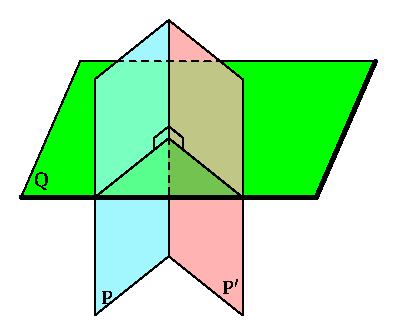
\includegraphics[scale=1]{fig2c_espace.6}
	\end{center}
	
	\begin{center}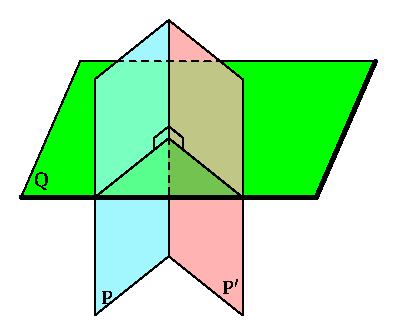
\includegraphics[scale=1]{fig2c_espace.8}\end{center}
	
	\begin{center} 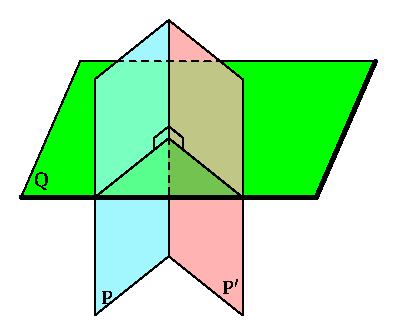
\includegraphics[scale=1]{fig2c_espace.10}\end{center}
	
	\begin{center}
\newrgbcolor{ccqqqq}{0.8 0 0}
\newrgbcolor{zzttqq}{0.6 0.2 0}
\psset{xunit=1.0cm,yunit=1.0cm,algebraic=true,dotstyle=o,dotsize=3pt 0,linewidth=0.8pt,arrowsize=3pt 2,arrowinset=0.25}
\begin{pspicture*}(-4.16,0.46)(5.8,7.74)
\pspolygon[linestyle=none,fillstyle=solid,fillcolor=zzttqq,opacity=0.1](-1.74,2.98)(-0.2,4.19)(1.44,4.21)(1.54,3.02)
\psline[linestyle=dotted](-1.74,2.98)(1.54,3.02)
\psline[linestyle=dotted](1.54,3.02)(2.62,1.58)
\psline(2.62,1.58)(-0.66,1.54)
\psline(-0.66,1.54)(-1.74,2.98)
\psline(-1.74,2.98)(0.26,6.84)
\psline(1.54,3.02)(0.26,6.84)
\psline(0.26,6.84)(-0.66,1.54)
\psline(0.26,6.84)(2.62,1.58)
\psplot[linecolor=ccqqqq]{-4.16}{5.8}{(-13.75-0.04*x)/-3.28}
\psplot[linecolor=ccqqqq]{-4.16}{5.8}{(-5.08-0.04*x)/-3.28}
\psline[linestyle=dotted,linecolor=zzttqq](-1.74,2.98)(-0.2,4.19)
\psline[linecolor=zzttqq](-0.2,4.19)(1.44,4.21)
\psline[linestyle=dotted,linecolor=zzttqq](1.44,4.21)(1.54,3.02)
\psline[linestyle=dotted,linecolor=zzttqq](1.54,3.02)(-1.74,2.98)
\rput[bl](-0.9,1.26){$A$}
\rput[bl](2.4,1.24){$B$}
\rput[bl](1.4,2.66){$C$}
\rput[bl](-2.04,2.72){\darkgray{$D$}}
\rput[bl](0.34,6.96){$S$}
\rput[bl](-0.12,4.3){\darkgray{$I$}}
\rput[bl](-2.46,3.76){\ccqqqq{$d$}}
\end{pspicture*}
\end{center}

\begin{center} 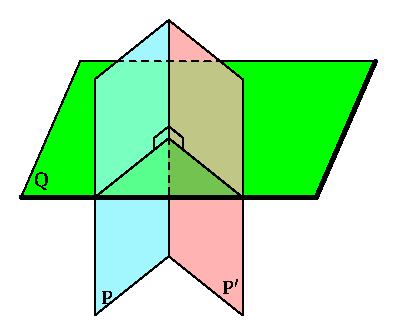
\includegraphics[scale=1]{fig2c_espace.9}\end{center}

\begin{center} 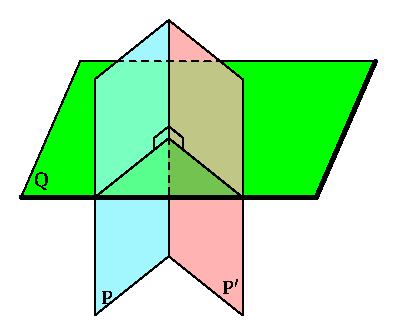
\includegraphics[scale=1]{fig2c_espace.11}\end{center}

\begin{center} 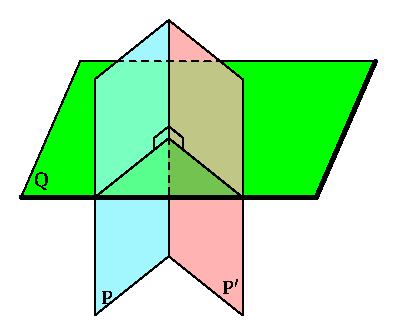
\includegraphics[scale=1]{fig2c_espace.12}\end{center}
\end{document}